\section{Playlist Generation} % (fold)
\label{sec:playlist_generation}

This section details the \'practical\' application of our data mining efforts. First, the section will detail
the overall concept of creating a bridgin playlist between two songs. Next, we will describe the algorithms used in our applications. And finally, we will discuss the possibilities of the playlist.

\subsection{Concept}
By using an ESOM to cluster and project our data set, we can use the two-dimensional grid of neurons to create paths between songs. A \'bridging playlist\' is found by creating a path between two neurons on the grid and relating songs in our data set to neurons on the path. The path is the shortest path between two neurons with each neuron having a connection to its adjacent neurons. The playlist generation can be explained with the following steps:
\begin{itemize}
\item Select two songs from a list and identify their bestmatch neurons on the grid, \\
\item Let each neuron $ n_{k,i} $  have the property that it is connected to neurons $ [ n_{k+1,i} ; n_{k-1,n} ; n_{k,n+1} ; n_{k,n-1} ], $ \\
\item Create a shortest path from the previously selected bestmatch neurons, \\
\item Delete any neuron from the path that is not a bestmatch neuron, \\
\item Associate bestmatches with songs that constitute the playlist
\end{itemize}

This description of the concept presents two important challenges. First, how do we weigh each connection from neuron to neuron, and second, how do we associate bestmatch neurons with songs that qualify to fit the playlist?
These challenges are addressed next in the algorithms section.\\

\subsection{Algorithms}

To address the first challenge of connecting neurons and finding a path between them, we use a popular mode of abstraction: graph building and shortest path finding in graphs. We use a standard adjacency list based graph CITATION that represent nodes as vertices and connections between nodes as edge. Each edge is weighted by calculating the euclidean distance between the prototype vectors of each neuron. \\
Creating a path between two bestmatch neurons is then done by using Dijkstra\'s shortest path algorithm for non-negative weighted graphs CITATION. We will claim but not prove that if the graph is built properly, this algorithm will find the shortest path (if it exists) between two nodes. \\

Applying the algorithm to the ESOM yields a list of bestmatch neurons. This list must then be associated with songs that originally made the bestmatch neuron fire. In order for us to do this, we log each song-to-neuron of the final epoch of the ESOM training. This, however, may still yield a list of several songs on each bestmatch, depending on clustering, ESOM size and song similarity. \\
Choosing from these songs is then done by using the K-Nearest Neighbours (KNN) algorithm CITATION. K-Nearest is mainly used for classifying and predicting new sets of data, but since it's essentially an algorithm for finding the $k$ closest points in a space, we can use it to choose songs that fit our playlist. Our method for doing so is as follows:

\begin{itemize}
\item Starting with a list $ n_1, n_2, \dots, n_k $ , and their associated lists $ l_1, l_2, \dots, l_n $ where $n$ denotes a step on the path between two songs and $l$ denotes songs on that particular step: \\
\item Select $ n_{i+1} $ from $ l_{i+1} $ with KNN such that the source song of the algorithm is what was chosen in the $ n{i} $ step \\
\item Either select $K = 1$ in KNN or pick one of the songs from the result of the previous KNN iteration and continue until $n_k$ is reached.\\
\end{itemize}

\begin{figure}[htb!]
	\centering
	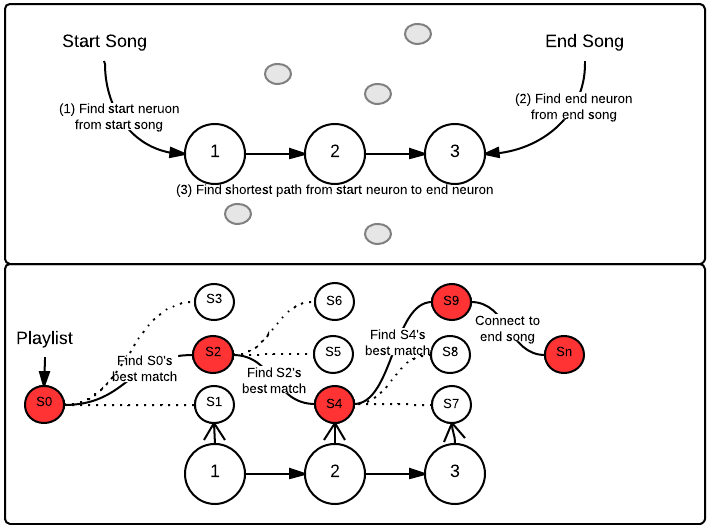
\includegraphics[width=\textwidth]{figures/playlist-generation}
	\caption{Illustration of the playlist generation. First, the start and end songs are mapped to the neurons that contain them. Then a shortest path is found between the neurons. Starting from the start song \(S0\) the KNN is found in the set of songs represented by the next neuron. This is continued until the next neuron is end neuron. The playlist is finished with the end song.}
\end{figure}

By using KNN, we attempt to smoothen the transition between each possible song result. \\
The final thing we will discuss in the algorithms section is the choice of basis for our graph. By default, we chose 
the prototype vectors of the ESOM and the distance between them as the edges in the graph. However, an alternative solution is to use the heights of the U-Matrix as the edges between neurons. The results are very similar, which is expected as the heights of the U-Matrix are the average distance to adjacent neurons. However, the actual songlist produced by the KNN song is strikingly different. We present the results in the following section.

\subsection{Results}

We present two different results of the playlist generation: the results of using the ESOM weights as the basis for our graphs and the results for 





% section playlist_generation (end)